%%%%%%%%%%%%%%%%%%%%%%%%%%%%%%%%%%%%%%
% LaTeX poster template
% Created by Nathaniel Johnston
% August 2009
% http://www.nathanieljohnston.com/index.php/2009/08/latex-poster-template/
%%%%%%%%%%%%%%%%%%%%%%%%%%%%%%%%%%%%%%

\documentclass[final]{beamer}
\usepackage[scale=1]{beamerposter}
\usepackage{graphicx}			% allows us to import images
\usepackage{subfig}       % to put figures side by side
\usepackage{amsmath}
\usepackage{amsfonts}
\usepackage{booktabs}
%-----------------------------------------------------------
% Define the column width and poster size
% To set effective sepwid, onecolwid and twocolwid values, first choose how many columns you want and how much separation you want between columns
% The separation I chose is 0.024 and I want 4 columns
% Then set onecolwid to be (1-(4+1)*0.024)/4 = 0.22
% Set twocolwid to be 2*onecolwid + sepwid = 0.464
%-----------------------------------------------------------

\newlength{\sepwid}
\newlength{\onecolwid}
\newlength{\twocolwid}
\newlength{\threecolwid}
\setlength{\paperwidth}{120cm}
\setlength{\paperheight}{90cm}
\setlength{\sepwid}{0.02\paperwidth}
\setlength{\onecolwid}{0.31\paperwidth}
\setlength{\twocolwid}{0.66\paperwidth}
\setlength{\topmargin}{-0.5in}
\usetheme{confposter}

%-----------------------------------------------------------
% Define colours (see beamerthemeconfposter.sty to change these colour definitions)
%-----------------------------------------------------------

\setbeamercolor{block title}{fg=ngreen,bg=white}
\setbeamercolor{block body}{fg=black,bg=white}
\setbeamercolor{block alerted title}{fg=white,bg=dblue!70}
\setbeamercolor{block alerted body}{fg=black,bg=dblue!10}

% MATH -----------------------------------------------------------
\newtheorem{thm}{Theorem}[section]
\newtheorem{cor}[thm]{Corollary}
\newtheorem{lem}[thm]{Lemma}
\newtheorem{prop}[thm]{Proposition}
\theoremstyle{definition}
\newtheorem{defn}[thm]{Definition}
\newtheorem{stasss}[thm]{Standing Assumption}
\theoremstyle{remark}
\newtheorem{rem}[thm]{Remark}
\newtheorem{exa}[thm]{Example}

\newcommand{\norm}[1]{\left\Vert#1\right\Vert}
\newcommand{\abs}[1]{\left\vert#1\right\vert}
\newcommand{\set}[1]{\left\{#1\right\}}
\newcommand{\Real}{\mathbb R}
\newcommand{\Natural}{\mathbb N}
\newcommand{\Complex}{\mathbb C}
\newcommand{\eps}{\varepsilon}
\newcommand{\To}{\longrightarrow}
\newcommand{\BX}{\mathbf{B}(X)}
\newcommand{\A}{\mathcal{A}}
\newcommand{\such}{\, | \, }
% PROBABILITY ----------------------------------------------------
\newcommand{\prob}{\mathbb{P}}
\newcommand{\Exp}{\mathcal E}
\newcommand{\parti}{\mathbb{T}}
\newcommand{\Time}{\mathfrak{T}}
\newcommand{\Timestar}{\Time{[0, \tau^*]}}
\newcommand{\oTime}{\overline{\Time}}
\newcommand{\oE}{\overline{E}}
\newcommand{\ove}{\overline{e}}
\newcommand{\qprob}{\mathbb{Q}}
\newcommand{\expec}{\mathbb{E}}
\newcommand{\expecp}{\expec_\prob}
\newcommand{\expecq}{\expec_\qprob}
\newcommand{\var}{\mathrm{var}}
\newcommand{\cov}{\mathrm{cov}}
\newcommand{\corr}{\mathrm{cor}}
\newcommand{\probtriple}{(\Omega, \mathcal{F}, \prob)}
\newcommand{\basis}{(\Omega,  \, (\F_t)_{t \in \Real_+}, \, \prob)}
\newcommand{\filtration}{\mathbf{F} = \pare{\mathcal{F}_t}_{t \in \Real_+}}
\newcommand{\F}{\mathcal{F}}
\newcommand{\G}{\mathcal{G}}
\newcommand{\cadlag}{c\`adl\`ag\,}
\newcommand{\caglad}{c\`agl\`ad}
\newcommand{\ud}{\mathrm d}
\newcommand{\inner}[2]{\langle #1 , #2 \rangle}
% MISC -----------------------------------------------------------
\newcommand{\liminfn}{\liminf_{n \to \infty}}
\newcommand{\limsupn}{\limsup_{n \to \infty}}

\newcommand{\limn}{\lim_{n \to \infty}}

\newcommand{\plim}{{\prob \textrm{-} \lim}}
\newcommand{\plimn}{\plim_{n \to \infty}}



\newcommand{\ttau}{{\widetilde{\tau}}}
\newcommand{\otau}{{\overline{\tau}}}


\newcommand{\uS}{\underline{S}}
\newcommand{\oS}{\overline{S}}

\newcommand{\uC}{\underline{\mathcal{C}}}
\newcommand{\oC}{\overline{\mathcal{C}}}



\newcommand{\pare}[1]{\left(#1\right)}
\newcommand{\bra}[1]{\left[#1\right]}
\newcommand{\cbra}[1]{\left\{#1\right\}}
\newcommand{\dbra}[1]{[\kern-0.15em[ #1 ]\kern-0.15em]}
\newcommand{\dbraco}[1]{[\kern-0.15em[ #1 [\kern-0.15em[}
\newcommand{\dbraoc}[1]{]\kern-0.15em] #1 ]\kern-0.15em]}

\newcommand{\og}{\overline{g}}




\newcommand{\dfn}{\, := \,}


\newcommand{\htau}{\widehat{\tau}}



\newcommand{\indic}{\mathbb{I}}

\newcommand{\tsigma}{\widetilde{\sigma}}
\newcommand{\wh}[1]{\widehat{#1}}

\newcommand{\X}{\mathcal{X}}
\newcommand{\C}{\mathcal{C}}
\newcommand{\bL}{\mathbb{L}}
\newcommand{\cL}{\mathcal{L}}
\newcommand{\cT}{\mathcal{T}}
\newcommand{\D}{\mathcal{D}}
\newcommand{\fR}{\mathfrak{R}}
\newcommand{\fM}{\mathfrak{M}}
\newcommand{\fH}{\mathfrak{H}}
\newcommand{\fC}{\mathfrak{C}}
\newcommand{\fs}{\mathfrak{s}}
\newcommand{\fv}{\mathfrak{v}}
\newcommand{\ey}{{}^\epsilon \kern-0.15em Y}
\newcommand{\ev}{{}^\epsilon \kern-0.15em V}
\newcommand{\eM}{{}^\epsilon \kern-0.27em M}
\newcommand{\wt}[1]{\widetilde{#1}}

\newcommand{\com}[1]{{ \color{blue} \textbf{[#1]} }}


\newcommand{\esssup}[1]{{\text{esssup}_{#1}}}

%-----------------------------------------------------------
% Name and authors of poster/paper/research
%-----------------------------------------------------------

\title{Empirical Asset Pricing through Machine Learning}
\author{Hao Xing}
\institute{Boston University}

%-----------------------------------------------------------
% Start the poster itself
%-----------------------------------------------------------
% The \rmfamily command is used frequently throughout the poster to force a serif font to be used for the body text
% Serif font is better for small text, sans-serif font is better for headers (for readability reasons)
%-----------------------------------------------------------

\usepackage{exscale}

\begin{document}
\begin{frame}[t]
 \begin{columns}[t]												% the [t] option aligns the column's content at the top

  \begin{column}{\sepwid}\end{column}			% empty spacer column

    \begin{column}{\onecolwid}

      \begin{block}{Introduction}
        \rmfamily{In a Markovian stochastic volatility model, the value function of a European contingent claim is the expectation of the terminal payoff under a (local) martingale measure, conditioning on the market's current configuration. Heuristically, this value function satisfies a PDE, which we call the \emph{valuation equation}. Even though the intuition is clear, it is surprisingly tricky to rigorously prove the heuristic connection, because

        \vskip1ex

        \begin{itemize}
         \item Volatility may vanish on the boundaries of state space. Then the standard Feynman-Kac formula cannot be applied.
         \item The asset-price process can be a \emph{strict local martingale}; see [1]. Then the valuation equation may have multiple solutions; see [4].
        \end{itemize}


        \vskip1ex

        We focus on the following questions in stochastic volatility models:

         \vskip1ex

        \begin{itemize}
	       \item What is the concept of a solution (regarding smoothness and boundary conditions) such that the value function is one such solution?
           \item What is a natural condition under which the value function is the unique solution?
           \item When the uniqueness in fails, how could one identify the value function among all possible solutions?
        \end{itemize}

        The above questions have been discussed in [2], [3] and etc. We assume minimal assumptions on the stochastic volatility models, which may have various behaviors:

        \vskip1ex

        \begin{itemize}
         \item The volatility can potentially reach zero.
         \item The asset-price can be a strict local martingale.
         \item The boundary condition to the valuation equation may be unnecessary.
         \item The payoff function can be unbounded.
        \end{itemize}
        }
      \end{block}

      \vskip2ex

      \begin{block}{The stochastic volatility model}
       \rmfamily{On a filtered probability space $\basis$, the model has the following dynamics:
       \begin{align*}
        dS_t &= S_t \, b(Y_t) \,dW_t, \quad S_0 = x \in \Real_{+}, \\
        dY_t &= \mu(Y_t) \,dt + \sigma(Y_t) \,dB_t, \quad Y_0 = y \in \Real_{+},
       \end{align*}
       where $W$ and $B$ are two Wiener processes with constant correlation $\rho\in (-1,1)$.

       \vskip1ex

       \textbf{Standing assumption}: (satisfied by most models in practice)
        \begin{enumerate}
            \item[(i)] $\mu: \Real_+ \rightarrow \Real$ is locally Lip. and $\mu(0) \geq 0$. $\sigma: \Real_+ \rightarrow \Real_+$ is locally $(1/2)$-H\"{o}lder, strictly positive on $\Real_{++}$, and satisfies $\sigma(0)=0$. Also,
                \begin{equation*}
                    |\mu(y)| + \sigma(y) \leq C(1+y) \quad \text{ for } y\in \Real_+.\label{eq: mu sigma linear}
                \end{equation*}
            \item[(ii)] $b: \Real_+ \rightarrow \Real_+$ satisfies $b(y)>0$ for $y\in \Real_{++}$ and $b(0)=0$. $b$ is locally $\alpha$-H\"{o}lder, and $\sigma b$ is locally Lip. $b$ has at most polynomial growth.
        \end{enumerate}
        }
      \end{block}

      \begin{block}{Zero volatility}
     \rmfamily{
      For $y \in \Real_+$, we define $\tau^y_0 := \inf\set{t \in \Real_{++} \such Y^y_t =0}$.
      \begin{itemize}
	       \item when $\mu(0)=0$, $Y^y_t = 0$ for $\tau^y_0 \leq t < \infty$, thus $0$ is \emph{absorbing};
	       \item when $\mu(0)>0$, $Y^y$ is lead back into $\Real_{++}$ after $\tau^y_0$.
      \end{itemize}

      \vskip1ex

      \textbf{Lemma}:
        Fix $y \in \Real_+$. If $\mu(0)>0$, then $\int_{\Real_+} \indic_{\set{Y^y_t = 0}} d t= 0$.

      \vskip1ex

      In this case the point $0$ is \emph{instantaneously reflecting}.
     }
     \end{block}
    \end{column}

    \begin{column}{\onecolwid}
     \begin{block}{Martingale property of the asset-price}
      \rmfamily{
      Let us consider an auxiliary diffusion $\wt{Y}$:
      \begin{equation*}
        d\wt{Y}_t = (\mu+ \rho b \sigma) (\wt{Y}_t) \, dt + \sigma(\wt{Y}_t) \, d B_t, \quad \wt{Y}_0=y.
      \end{equation*}

      \vskip2ex

      \textbf{Proposition}: The following statements are equivalent:
      \begin{enumerate}
       \item[(i)] $S^{x,y}_{\cdot \wedge T}$ is a strict local martingale for some, then all, $(x,y,T)\in \Real^3_{++}$.
       \item[(ii)] $\wt{Y}$ \emph{explodes} to $\infty$ in finite time.
       \item[(iii)] $\fv(\infty) = \infty$.
      \end{enumerate}

      \vskip2ex

      Here $\fv(y) := \int_c^{y} \frac{\fs(y) - \fs(\xi)}{\fs'(\xi) \sigma^2(\xi)} \, d \xi$ for $y \in \Real_{++}$, where $\fs$ is the scale function for the diffusion $\wt{Y}$.

      \vskip2ex

      \textbf{Remark}: This proposition uses Sin's argument in [6]. But its statement is stronger than the one in [6]. It says that in a time-homogeneous model, if $S$ is going to lose its martingale property eventually, it must lose it immediately. This proposition also generalizes Theorem~2.4 in [5].
      }
     \end{block}

     \begin{block}{The valuation equation}
     \rmfamily{
      Given a continuous payoff $g: \Real_+^2 \rightarrow \Real_+$ with $g(x,y)\leq C(1+x+y^m)$.

      The value function of a European option is defined via
      \[
       u(x,y,T) := \expec\bra{g\pare{S^{x,y}_T, Y^y_T}}, \quad \text{ for } (x,y,T) \in \Real_+^3.
      \]
      $u$ grows at most linear in $x$ and poly. in $y$.

      \vskip2ex

      The valuation equation is
      \vskip1ex

      \begin{equation}\label{eq: pricing eq} \tag{VE}
        \begin{split}
        & \partial_T u (x,y,T) = \cL v (x,y,T), \quad (x,y,T) \in \Real_{++}^3,\\
        & u(x,y,0) = g(x,y), \quad (x,y)\in \Real_+^2,
        \end{split}
        \end{equation}

      \vskip1ex

        in which $\cL$ is the infinitesimal generator of $(S, Y)$:
        \[
        \cL := \mu(y) \partial_y + \frac12 b^2(y) x^2 \partial^2_{xx} +  \frac12 \sigma^2(y) \partial^2_{yy}  + \rho b(y) \sigma(y) x \partial^2_{x y}.
        \]

        Note that $\cL$ degenerates at $y=0$ to the operator $\mu(0)\partial_y$.

        \vskip2ex

        \textbf{Boundary conditions}:
        \begin{itemize}
         \item When the boundary is absorbing, $v(x,0,T) = g(x,0)$ needs to be satisfied.
         \item When the boundary is instantaneously reflecting, one usually chooses
         \begin{equation}\label{BC}
          \partial_T v(x,0,T) = \mu(0) \partial_y v(x,0,T). \tag{BC}
         \end{equation}
        \end{itemize}

        \vskip2ex

        \textbf{Definition}:A function $v\in C(\Real_+^3) \cap C^{2,2,1}(\Real_{++}^3)$, that solves (VE), is called a \emph{classical solution} in all the following cases (below, $y$ is arbitrary in $\Real_{++}$):
        \begin{enumerate}
            \item[(A)] When $\prob[\tau^y_0=\infty]=1$.

            \item[(B)] When $\prob[\tau^y_0<\infty] >0$, $\mu(0)=0$, and $v$ satisfies $v(x,0,T) = g(x,0)$.

            \item[(C)] When $\prob[\tau^y_0<\infty]>0$, $\mu(0)>0$, and $v$ belongs to
            \[
            \begin{split}
                \fC := &\left\{ f \in C(\Real_+^3) \cap C^{2,2,1}(\Real_{++}^3) \such \text{all } \partial_T f, \  \partial_y f, \ y^{2 \alpha}
                \partial^2_{xx} f \right. \\
                & \left. \text{ are locally bounded on } \Real_{++} \times \Real_+ \times \Real_{++}\right\}.
            \end{split}
            \]
            For any $f\in C(\Real_+^3) \cap C^{2,2,1}(\Real_{++}^3)$, by saying that $\partial_T f, \  \partial_y f$, and $\ y^{2 \alpha} \partial^2_{xx} f$ are locally bounded on $y=0$, we mean that
            \[
                \limsup_{y \downarrow 0} \sup_{(x, T) \in [n^{-1}, n]^2} \bra{|\partial_T f| + |\partial_y f| + y^{2 \alpha} |\partial^2_{xx} f| }  < \infty
            \]
            holds for all $n \in \Natural$.
            \end{enumerate}
     }
     \end{block}
    \end{column}

    \begin{column}{\onecolwid}
        \begin{block}{value-weighted portfolio}
         \rmfamily{
            \textbf{Reasons for value-weighted portfolio construction}:
            \begin{enumerate}
                \item[(i)] We choose value-weighted portfolios because stocks with a large market value of equity are often “important” stocks that are traded and held by a large number of people. We want to measure the performance of our models while targeting those important assets.
                \item[(ii)] The target of our model is to forecast the return of each permno, however, in real life, people often focus on the return of a portfolio rather than single stocks. Thus we also need to measure the performance of simple portfolios to get a better understanding of the performance of our models.
            \end{enumerate}
            \vskip1ex
            \textbf{Details of portfolio construction process}: We only construct portfolios for gbrt, random forest as well as neural network models as these models have significantly higher out-of-sample $R^2$ than other models. We set the transaction cost to be 2\% and use the S\&P500 index as the benchmark. Given the models' predicted returns and the market equity of each permno, we first rank the permnos by their predicted returns, then we select the 50 permnos that have the highest average return as the stocks to buy, and the 50 permnos that have the lowest average return as the stocks to sell, and weight each permno according to their market equity. Doing so, we now have a long-only portfolio and a short-only portfolio for each model, we then combine them to make a long-short portfolio for each model.
            \vskip1ex
            \textbf{Result}: while the neural network model has bad performance, the gbrt model and random forest model have relatively good performance and can beat the benchmark.
            \begin{figure}
              \centering
              \subfloat[\centering cumulative return of long-short portfolios]{{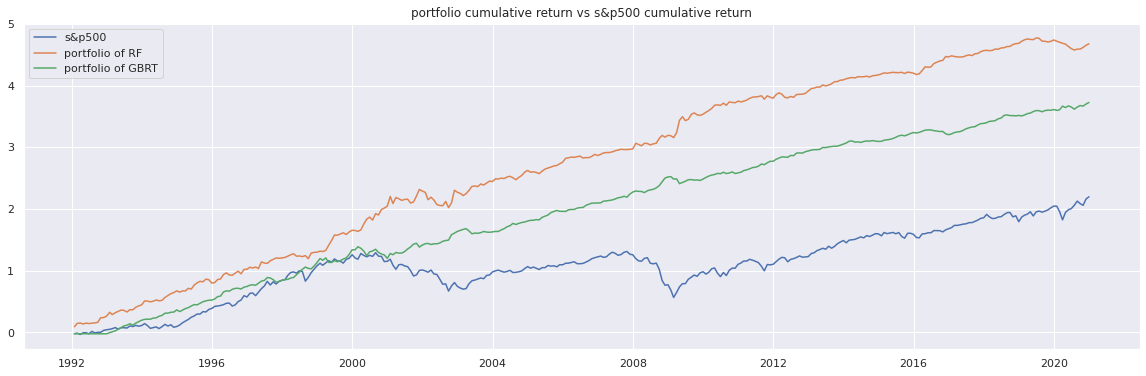
\includegraphics[width=0.44\linewidth]{picture_folder/gbrt_n_rf_output.png} }}
              \quad
              \subfloat[\centering monthly return of long-short portfolios]{{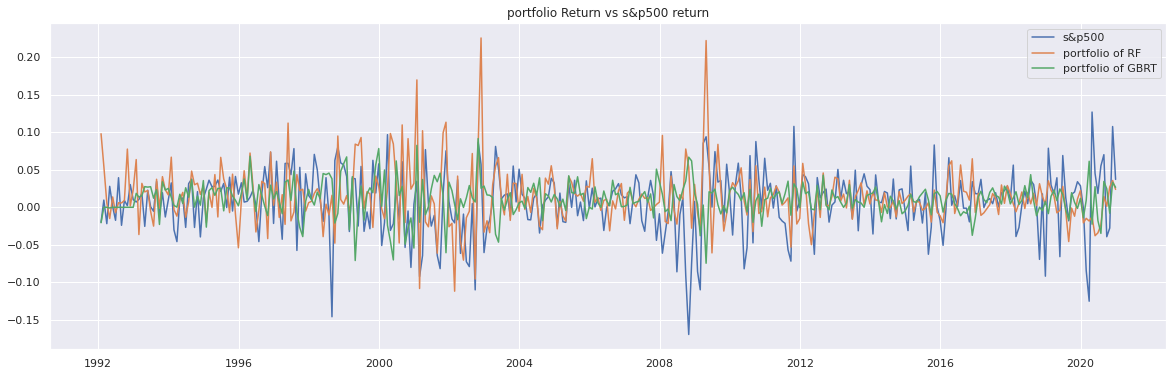
\includegraphics[width=0.44\linewidth]{picture_folder/val.png} }}
              \label{fig:portfolio_return}
          \end{figure}
            \vskip2ex
          As we can see, the portfolio based on the predicted returns of random forest model has the hightest cumulative return. However, the sharpe ratio(annualized) of random forest's portfolio is around 1.27, which is smaller then the sharpe ratio of gbrt's portfolio, which is around 3.28. 
          \begin{table}[]
            \caption{the SR, IR, MDD of each model}
            \label{tab:sr_n_ir_n_md}
            \vspace{-15mm}
            \resizebox{\columnwidth}{!}{%
            \begin{tabular}{@{}llll@{}}
            \toprule
            \textbf{MODELS} &
              annualized sharpe ratio &
              \begin{tabular}[c]{@{}l@{}}annualized information ratio\\ (with the benchmark of S\&P500 index)\end{tabular} &
              maximum drawdown \\ \midrule
            neural network & 0.921811 &          &           \\
            random forest  & 3.275392 & 0.530446 & -0.283552 \\
            gbrt           & 1.269521 & 1.048854 & -0.228834 \\ \bottomrule
            \end{tabular}%
            }
            \end{table}
        }
        \end{block}

        \begin{block}{conclusion}
         \rmfamily{
            \textbf{Main theorem}:
            The value function $u \in C(\Real_+^3) \cap C^{2,2,1}(\Real_{++}^3)$. Furthermore, $u$ is the smallest nonnegative classical solution to (VE) in each of the following cases (where $y$ is arbitrary in $\Real_{++}$):
            \begin{enumerate}
                \item[(A)] When $\prob[\tau^y_0 =\infty] =1$.
                \item[(B)] When $\prob[\tau^y_0 < \infty] >0$ and $\mu(0)=0$.
                \item[(C)] When $\prob[\tau^y_0<\infty] >0$, $\mu(0)>0$, and $u\in \fC$.
            \end{enumerate}
            In all of the above cases, the following two statements hold:
            \begin{enumerate}
            \item[(i)] If $g$ is strictly sublinear in $x$ and poly. in $y$, then $u$ is the unique classical solution within the same class of functions.

            \item[(ii)] If $g$ is linear growth in $x$ and poly. in $y$, then $u$ is the unique classical solution within the same class of functions \emph{if and only if} the  asset-price process is a martingale.
            \end{enumerate}
        }
        \end{block}

    \end{column}

 \end{columns}
\end{frame}
\end{document} 